\documentclass{article}
\usepackage{tikz}
\usepackage{float}
\usepackage{amsmath}
\usepackage{lmodern}
\usepackage{amssymb}
\usetikzlibrary{calc}
\usetikzlibrary{hobby}
\usetikzlibrary{decorations.markings}
\usetikzlibrary{patterns, patterns.meta}
\usetikzlibrary{shapes}
\usepackage{pgfplots}
\pgfplotsset{compat=1.18}
\begin{document}
\centering

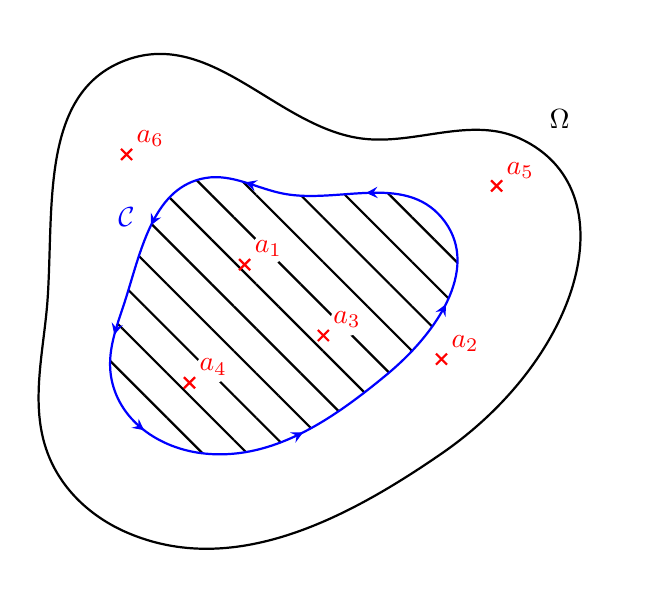
\begin{tikzpicture}
    \tikzset{
      cross/.style={cross out, draw=red, fill=none, minimum size=2*(#1-\pgflinewidth), inner sep=0pt, outer sep=0pt,line width = 0.8pt}, cross/.default={2.8pt},
    % style to apply some styles to each segment of a path
    on each segment/.style={
      decorate,
      decoration={
        show path construction,
        moveto code={},
        lineto code={
          \path [#1]
          (\tikzinputsegmentfirst) -- (\tikzinputsegmentlast);
        },
        curveto code={
          \path [#1] (\tikzinputsegmentfirst)
          .. controls
          (\tikzinputsegmentsupporta) and (\tikzinputsegmentsupportb)
          ..
          (\tikzinputsegmentlast);
        },
        closepath code={
          \path [#1]
          (\tikzinputsegmentfirst) -- (\tikzinputsegmentlast);
        },
      },
    },
    % style to add an arrow in the middle of a path
    mid arrow/.style={postaction={decorate,decoration={
          markings,
          mark=at position .5 with {\arrow[#1]{stealth}}
        }}},
  }
    % draw omega space
    \path [draw=black,thick]
    (2,-2) to[closed, curve through =
    { (-2,-3) (-3,-2) (-3,0) (-2,3) (1,2) }] (3,2);
    \draw[color=black] (3.5,2) node[above] {$\Omega$};

    % draw contour around poles
    \path [draw=blue,thick,pattern ={Lines[angle=135, distance=0.4cm]},postaction={on each segment={mid arrow=blue}},pattern ={Lines[angle=135, distance=0.4cm]}]
    (2,1) to[closed, curve through =
    { (0,1.3) (-1,1.5) (-2,0) (-2.2,-1) (-1,-2) }] (1.3,-1);
    \node at (-2,1) [draw=white, circle, inner sep=0, fill=white] {\textcolor{blue}{$\mathcal{C}$}};

    % draw poles
    \draw[color=red,thick] (-0.5, 0.4) node[cross] {};
    \node at (-0.2,0.6) [draw=white, circle, inner sep=0, fill=white] {\textcolor{red}{$a_1$}};

    \draw[color=red,thick] (2, -0.8)node[cross] {};
    \node at (2.3,-0.6) [draw=white, circle, inner sep=0, fill=white] {\textcolor{red}{$a_2$}};
    
    \draw[color=red,thick] (0.5, -0.5) node[cross] {};
    \node at (0.8,-0.3) [draw=white, circle, inner sep=0, fill=white] {\textcolor{red}{$a_3$}};
    
    \draw[color=red,thick] (-1.2, -1.1) node[cross] {};
    \node at (-0.9,-0.9) [draw=white, circle, inner sep=0, fill=white] {\textcolor{red}{$a_4$}};

    \draw[color=red,thick] (2.7, 1.4)node[cross] {};
    \node at (3,1.6) [draw=white, circle, inner sep=0, fill=white] {\textcolor{red}{$a_5$}};

    \draw[color=red,thick] (-2, 1.8)node[cross] {};
    \node at (-1.7,2) [draw=white, circle, inner sep=0, fill=white] {\textcolor{red}{$a_6$}};

\end{tikzpicture}
\end{document}